\documentclass[tikz,border=10pt]{standalone}
\begin{document}
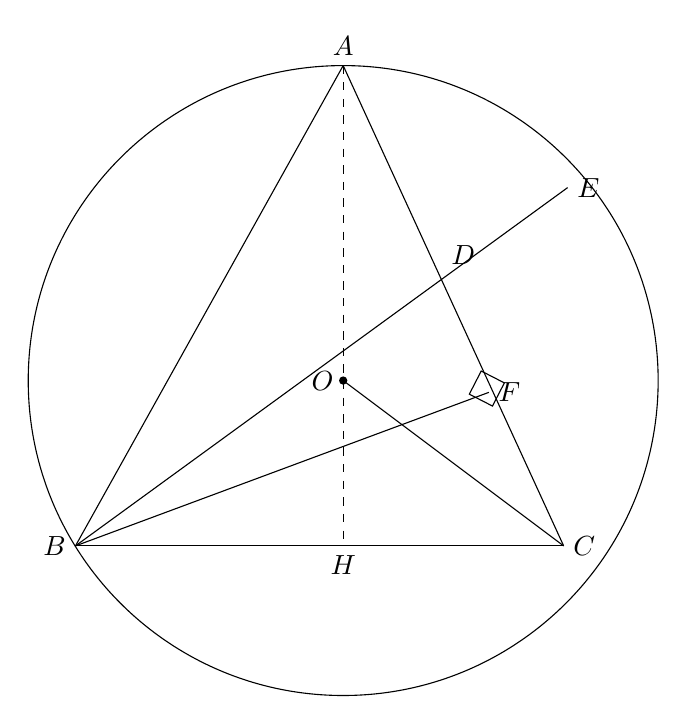
\begin{tikzpicture}[scale=1]

% Coordinates
\coordinate (O) at (0,0);
\coordinate (A) at (0,4);
\coordinate (B) at (-3.4,-2.1);
\coordinate (C) at (2.8,-2.1);
\coordinate (H) at (0,-2.1);
\coordinate (E) at (2.85,2.45);
\coordinate (D) at (1.25,1.35);
\coordinate (F) at (1.85,-0.15);

% Circle
\draw (O) circle[radius=4];

% Main triangle and chords
\draw (A) -- (B);
\draw (A) -- (C);
\draw (B) -- (C);
\draw (B) -- (E);
\draw (B) -- (F);
\draw (O) -- (C);

% Dashed altitude
\draw[dashed] (A) -- (H);

% Center point
\fill (O) circle[radius=1.5pt];

% Right-angle mark at F between BF and AC
\draw (1.602,-0.173) -- (1.753,0.121) -- (2.047,-0.030) -- (1.896,-0.324) -- cycle;

% Labels
\node[above] at (A) {$A$};
\node[left] at (B) {$B$};
\node[right] at (C) {$C$};
\node[below] at (H) {$H$};
\node[left] at (O) {$O$};
\node[right] at (E) {$E$};
\node[above right] at (D) {$D$};
\node[right] at (F) {$F$};

\end{tikzpicture}
\end{document}
